% Author:Zhengxin Tang(tang_zx@whu.edu.cn)
% 武汉大学物理学院硕博学位论文模板(https://github.com/tzxwhu/whu-physics-thesis-template)
% 在github上的武大毕业论文模板(https://github.com/whutug/whu-thesis)的基础上做了大量的修改,以符合最新的物院毕业论文模板要求(几乎全部)。在此,向原作者 WHU TeX User Group 致谢!!!
% 如果后续物院模板更新,则可联系作者做相应的修改。
 


%--------------------------------- tutorials----------------------------
% 以下仅列举了部分可能用到的设置选项,更多用法请参考文档《whuthesis.pdf》
% 论文具体内容的要求可以按照《武汉大学物理学院毕业论文格式3》

%----------------------------导言区开始分割线--------------------------------

\documentclass[type = master,class = academic]{whu-thesis}
% type: 可选项为 bachelor, master, doctor
% class: 可选项为 academic, professional
% showframe: 显示页面布局框架
% \PassOptionsToPackage{gbnamefmt = lowercase}{biblatex} % 英文作者姓名不强制大写


% 设置
\whusetup{
  info = {
    title      = {中文论文标题}, % 标题,可使用 \\ 手动换行
    title*     = {English title},
    department  = {物理科学与技术学院},
    department* = {School of Physics and Technology, Wuhan University},
    student_id = 0000000000000,% 学号
    author     = {张三},
    author*    = {San ZHANG},
    supervisor  = {李四},
    supervisor* = {Si LI},
    academic-title  = {教授},
    academic-title* = {Prof},
    %supervisor-outer = {}, % 校外导师(非必填)
    %supervisor-outer* = {}
    %academic-title-outer = {教授}, % 校外导师职称(非必填)
    subject = {}, % 学科名称(非必填)
    major   = {理论物理},
    major*  = {Theoretical Physics},
    research-area  = {弦论},
    research-area* = {String Theory},
    year = 2025, % 日期
    month = 8,
    keywords = {{关键词1};{关键词2};{关键词3};},
    keywords* = { {keyword1},{keyword2},{keyword3},},
    clc = O159, % 分类号
  },
  style = {
    % 字体相关选项
    font = times, % 西文字体,可选项为 default, times, xits, termes
    math-font = termes, % 数学字体,可选项为 default, xits, termes
    cjk-font = fandol, % 中文字体,可选项为 windows, mac, fandol(Linux/Overleaf/TexPage), sourcehan, none
    %cjk-fakefont = true, % 使用伪粗体与伪斜体
    % 参考文献及引用相关选项
    bib-backend = bibtex, % 参考文献引擎,可选项为 bibtex, biblatex
    bib-style = numerical, % 参考文献样式,可选项为 numerical, author-year
    %cite-style = <>, % 引用样式(自定义)
    bib-resource = {ref/refs.bib}, % 参考文献数据源
    % 页面相关选项
    chapter-page-header = true, % 章节首页是否有页眉
    % bachelor-encover = true, % 本科毕业论文英文封面
    library, % 图书馆模式(去掉论文中所有的空白页)
    license, % 使用授权协议书  
    % fullwidth-stop = true, % 句号样式
    % footnote-style = <>, % 脚注编号样式
    % abstract-keywords-type  = blankline, % 摘要与关键词之间样式,可选项为 blankline, newline, vfill
    % abstract-keywords-type* = blankline, % 摘要与关键词之间样式,可选项为 blankline, newline, vfill
  }
}
\whumodule{algorithm2e}

% =============================== 新命令======================================
% 在此设置所需的命令

% 修正:使用期刊全称
\newcommand{\apj}{The Astrophysical Journal}
\newcommand{\apjl}{The Astrophysical Journal Letters}  
\newcommand{\apjs}{The Astrophysical Journal Supplement Series}
\newcommand{\aj}{The Astronomical Journal}
\newcommand{\mnras}{Monthly Notices of the Royal Astronomical Society}
\newcommand{\aap}{Astronomy \& Astrophysics}
\newcommand{\araa}{Annual Review of Astronomy and Astrophysics}
\newcommand{\pasp}{Publications of the Astronomical Society of the Pacific}
\newcommand{\nat}{Nature}
\newcommand{\science}{Science}
\newcommand{\farcs}{\mbox{$.\!\!^{\prime\prime}$}} %arcsec






%--------------------------------导言区结束分割线--------------------------

% ==================================正文==================================
\begin{document}

\tableofcontents % 目录
% \listoffigures % 图目录
% \listoftables % 表目录

% 符号表
% \begin{notation}
%   $\omega_n$ & $n$-维欧氏空间中单位球的表面积 \\
%   $\alpha_n$ & $n$-维欧氏空间中单位球的体积 \\
% \end{notation}

\mainmatter
%在src文件夹中创建章节tex,在这里include。如需增加章节,按此方式即可;若删除章节,删除“src/.tex”文件,并在此处删除相应的\include{src/.tex}
\chapter{绪论}
\section{星系形态学}
星系形态学作为现代天文学和天体物理学的核心研究领域之一,为理解宇宙中最复杂的恒星系统~——~星系的形成与演化过程提供了重要的观测窗口\cite{Kormendy2004,Sandage2005,Mo2010,Conselice2014}。自Edwin Hubble在1926年首次建立系统性的星系分类体系\cite{Hubble1926}以来,并经由de Vaucouleurs等人的进一步发展和完善,星系形态学研究已经从最初的经验性分类发展成为连接观测天文学与理论天体物理学的重要桥梁。


\begin{figure}[htbp]
\centering
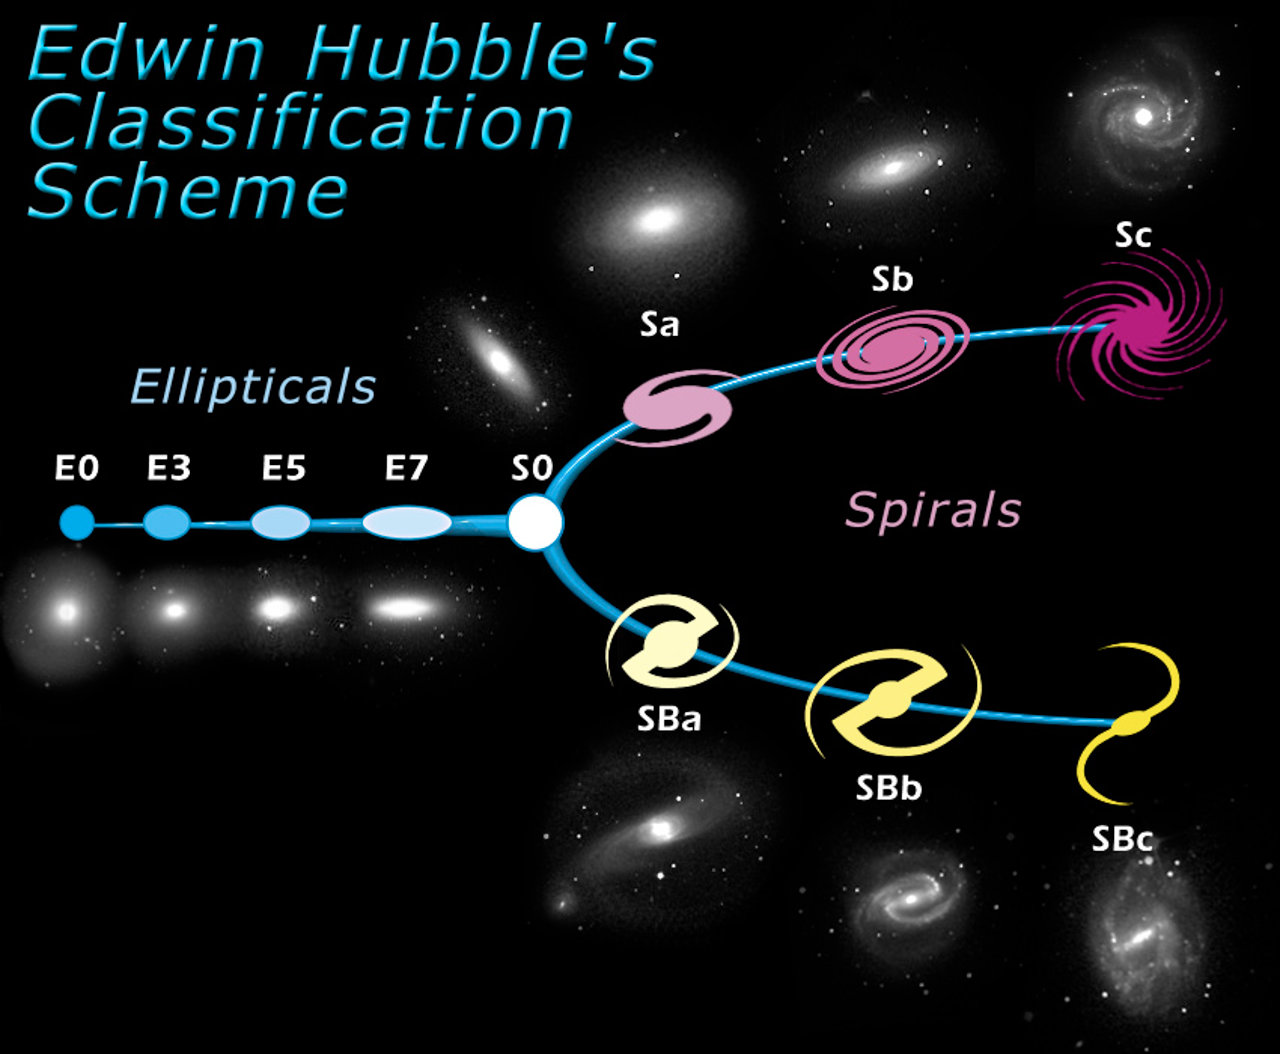
\includegraphics[width=0.45\textwidth]{Hubble_Sequence.jpg}
\caption{: \emph{Hubble Sequence示意图。左侧为椭圆星系序列(E0-E7),按照扁率递增排列,从近似球形(E0)到高度扁平(E7);中央为透镜状星系(S0),具有明显的核球和盘结构但缺乏螺旋臂特征;右侧分别为正常螺旋星系(Sa-Sc)和棒旋星系(SBa-SBc)序列,展现了从紧密缠绕的旋臂结构到疏松开放的旋臂形态的连续变化。图片来源:NASA\&ESA 。}}
\label{fig:hubble_sequence}
\end{figure}

所有参数的具体分布见表\ref{tab:simulation_parameters}:

\begin{table}[htbp]
\centering
\caption{模拟星系参数设置}
\label{tab:simulation_parameters}
\begin{tabular}{lc}
\hline
\hline
\textbf{参数} & \textbf{取值范围} \\
\hline
总星等 ($m_{\text{total}}$) & 20-28 AB mag \\
B/T比值 & 10\%-90\% \\
核球有效半径 ($R_{\text{bulge}}$) & 0\farcs05-0\farcs2 \\
盘有效半径 ($R_{\text{disc}}$) & 1.5-3.0 × $R_{\text{bulge}}$ \\
核球轴比 ($q_{\text{bulge}}$) & 0.8-0.9 \\
盘轴比 ($q_{\text{disc}}$) & 0.4-0.7 \\
核球Sérsic指数 ($n_{\text{bulge}}$) & 4.0 (固定) \\
盘Sérsic指数 ($n_{\text{disc}}$) & 1.0 (固定) \\
\hline
\hline
\end{tabular}
\end{table}

Sérsic轮廓作为描述星系表面亮度分布的核心数学工具,其一般形式可表示为:
\begin{equation}
I(R) = I_e \exp\left\{-k\left[\left(\frac{R}{R_{\text{eff}}}\right)^{1/n} - 1\right]\right\}
\end{equation}
\subsection{现代宇宙学框架下的星系形态演化}




\chapter{xxxx}

\section{xxxx}
\subsection{xxxx}
\chapter{xxxx}

\section{xxxx}
\subsection{xxxx}
\chapter{xxxx}

\section{xxxx}
\subsection{xxxx}
\chapter{xxxx}

\section{xxxx}
\subsection{xxxx}
\chapter{xxxx}

\section{xxxx}
\subsection{xxxx}

% 当然你也可以直接在这里写,不过这样不太方便管理
%\chapter{BBBB}


% 打印参考文献
\printbibliography

% 致谢
\begin{acknowledgements}
  对在课题研究及论文写作过程中给予指导和帮助的导师、校内外专家、实验技术人员、同学等表示感谢。
  
在致谢时建议具体,不同的人如何助力完成你的论文,都需要特别注明。如导师、其他老师或实验技术人员、以及同学对你论文的贡献是不一样的,有指引课题方向、修改论文,也有具体教会实验操作,也有协助你做了哪方向的实验,或者给你精神安慰、陪你度过紧张的研究生生涯。

越具体越能表达你真实的感受,否则就是毫无意义的套话。

对本研究开展得到经费支持的课题项目进行致谢,如国家自然科学基金、重点研发计划等。


\end{acknowledgements}



% 附录
\appendix
\ctexset{
  chapter/number = \arabic{chapter}
}

\chapter{答辩委员会决议}



\chapter{攻读硕士/博士学位期间取得的研究成果}
 \begin{enumerate}[label={[\arabic*]}]
  \item 
  \item 
  \item 
  \item 
  \item 
\end{enumerate}


\end{document}